\documentclass[11pt, a4paper]{article}

\usepackage[utf8]{inputenc}
\usepackage{authblk}
\usepackage{titlesec}

% Maths tools
\usepackage{amsmath}
\usepackage{amssymb}

% Margin
\usepackage[margin=2.9cm]{geometry}

% Line numbers
\usepackage{lineno}

%Scientific notation
\usepackage{siunitx}

% Spacing
\usepackage{setspace}
\doublespacing

% Enumeration
\usepackage{enumerate}

% indentation
\setlength\parindent{10pt}
\setlength{\parskip}{5pt}

% Figures
\usepackage{graphicx}
\usepackage{caption}
\usepackage{subcaption}
\usepackage{epstopdf}
\renewcommand{\thefigure}{\textbf{\arabic{figure}}}
\renewcommand{\figurename}{\textbf{Supplementary Figure}}

%table
\usepackage{multirow}
\usepackage{hhline}
\usepackage[table]{xcolor}
\renewcommand{\thetable}{\textbf{\arabic{table}}}
\renewcommand{\tablename}{\textbf{Supplementary Table}}

%footnotes
\usepackage{footmisc}
\renewcommand{\thefootnote}{\fnsymbol{footnote}}

% References
\usepackage[sort&compress, numbers,super]{natbib}
\bibliographystyle{unsrtnat}
\PassOptionsToPackage{hyphens}{url}\usepackage[colorlinks=true,linkcolor=magenta, citecolor=magenta]{hyperref}
\renewcommand\refname{Supplementary References}

%subsubsection format
\titleformat*{\subsubsection}{\large\it}

%highlighting text
\usepackage{color, xcolor,soul}
\definecolor{blau}{RGB}{236,226,240}
\soulregister\cite7
\soulregister\citet7
\soulregister\citealt7
\soulregister\citenum7
\soulregister\citep7
\soulregister\ref7
\DeclareRobustCommand{\hlc}[1]{{\sethlcolor{blau}\hl{#1}}}

\usepackage{titlesec}% http://ctan.org/pkg/titlesec
\titleformat{\section}%
  [hang]% <shape>
  {\normalfont\bfseries\Large}% <format>
  {}% <label>
  {0pt}% <sep>
  {}% <before code>
  
\renewcommand{\thesection}{}% Remove section references...
\renewcommand{\thesubsection}{}%... from subsections
  \renewcommand{\thesubsubsection}{Supplementary Method \arabic{subsubsection}:}%... from subsections


  
%Title paper
\title{\vspace{-1cm} \normalsize Supplementary Information\\\vspace{0.2cm}
\LARGE Basic aspects of species' distributions}

\author{\textit{Bramon Mora and Alexander}}

\date{}

\begin{document}
\maketitle
\thispagestyle{empty}

\clearpage

\begin{figure}[ht]
  \centering
    \vspace{0.5cm}
    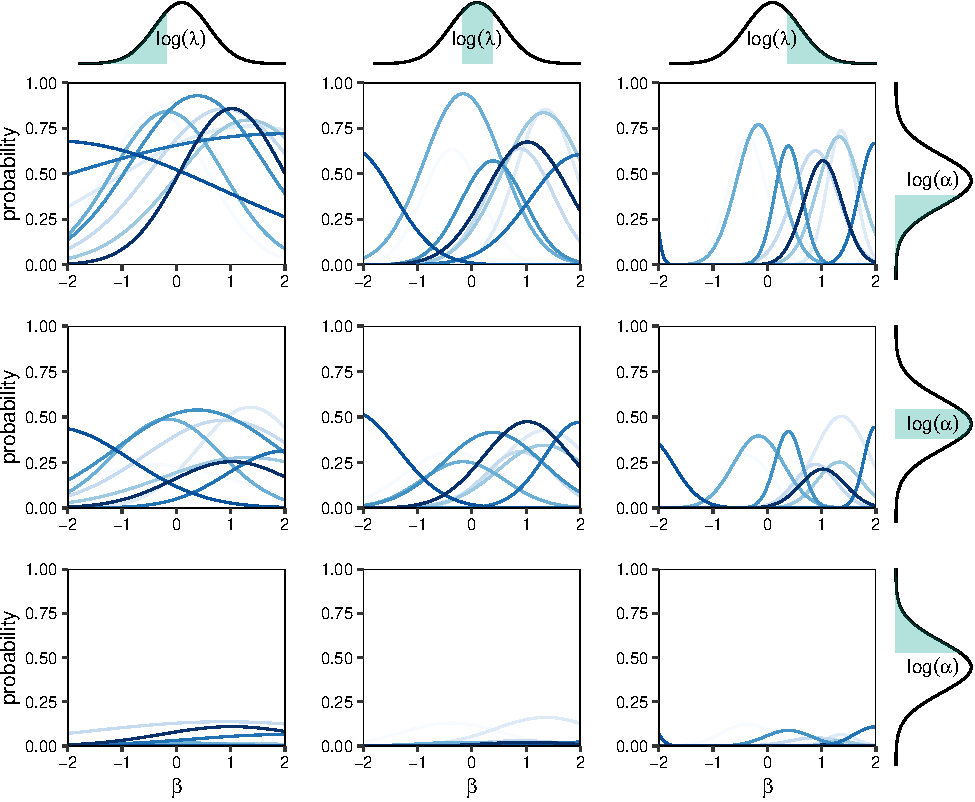
\includegraphics[width=1\textwidth]{figures/prior}
    	  \vspace{0.3cm}
	   \caption{Study of the priors for the baseline model presented in the main text.}
      \label{sfig:sensitivity}
\end{figure}

\clearpage

\begin{figure}[h]
  \centering
    \vspace{0.5cm}
    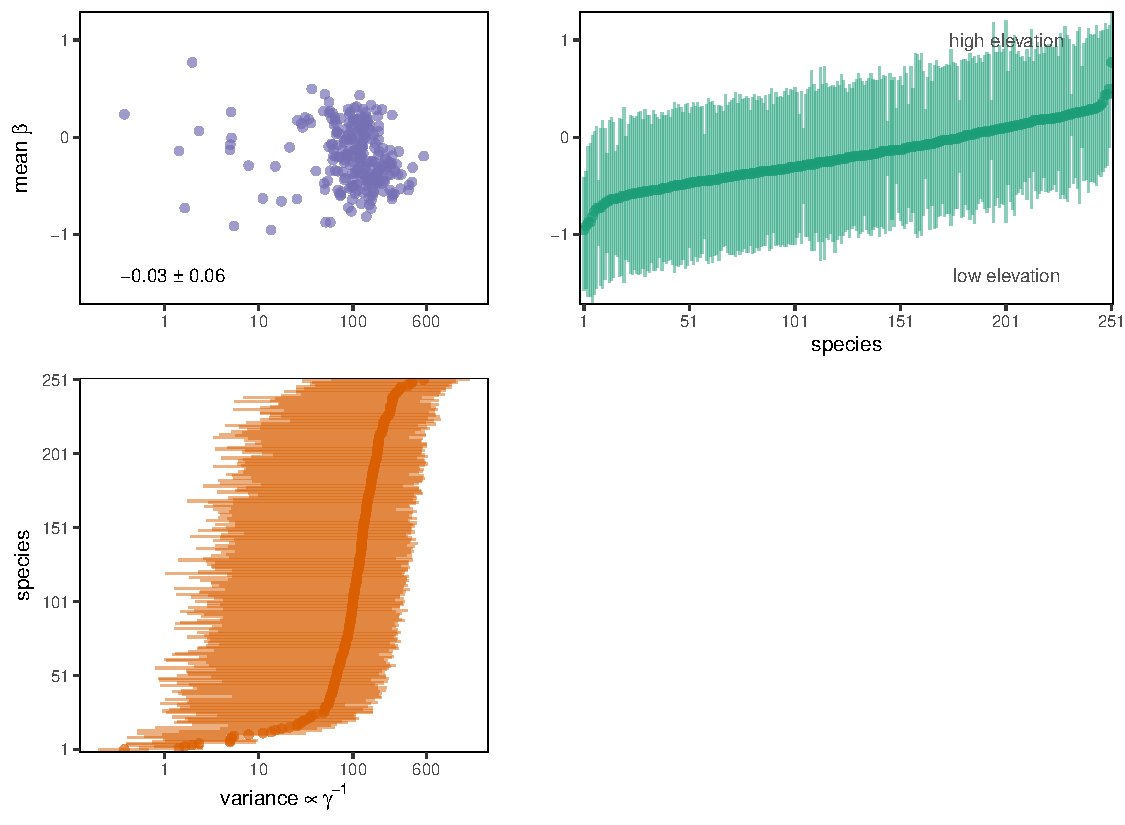
\includegraphics[width=1\textwidth]{figures/figure1-secondaxis}
    	  \vspace{0.3cm}
	   \caption{Relationship between mean and variance of species' distributions. These are the results for the second axis of variation for the climatic data.}
      \label{sfig:sensitivity}
\end{figure}

\clearpage

\bibliography{references_ab}

\end{document}
